\subsection{Healthy and diseased together}
In the previous sections it was demonstrated that the model works on samples from different datasets and performs well on both healthy and diseased samples it can be interesting to see how the model behave when both kinds of data are presented to it.
The goal of this part of work is to identify which genes or topics identify and distinguish tissues themselves and which drive cancer and are necessary to understand the differentiation between cancer types.

For this analysis data  from GTEx and TCGA were still analysed, but from a particular dataset available from~\cite{Wang2017} were authors tried to unify the normalization process from different dataset and sources~\cite{Betel2018}. This is, in practice, a mixed bigger dataset; note that not every tissue is present in both GTEx and TCGA, so only common tissues are considered here. The first label considered at this point is the tissue primary site, forgetting about its status (healthy or diseased), the secondary label refers to the tissues but separates their status. For example, a healthy brain sample from GTEx and a cancer brain from TCGA share the \textit{brain} primary site label but have different secondary site assignments.

Once the model is run, the first element to look at is the V-measure; in figure~\ref{fig:topic/merged/metric_scores_primarysite} the result for the primary site is quite satisfying: clusters are very homogeneous and V-measure's peak is near $0.8$.
\begin{figure}[htb!]
    \centering
    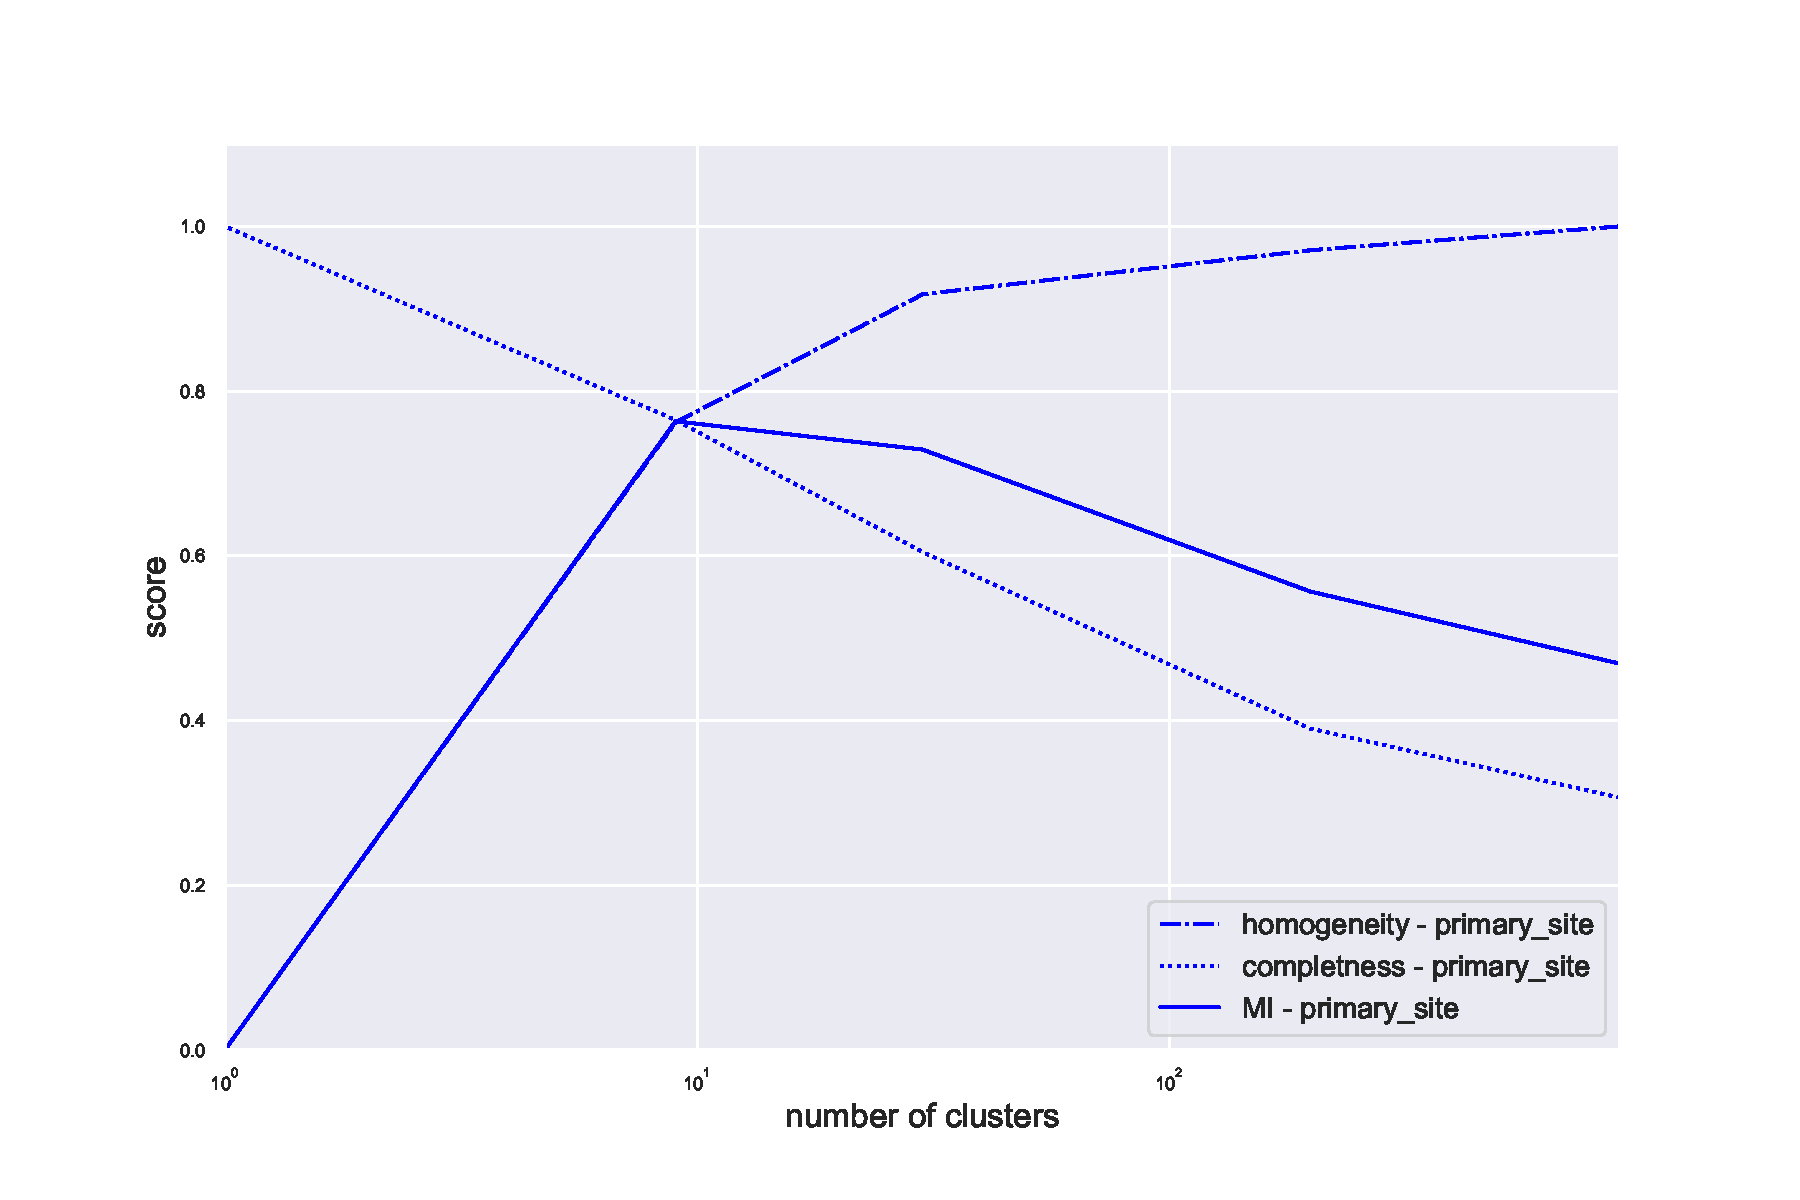
\includegraphics[width=0.8\linewidth]{pictures/topic/merged/metric_scores_primarysite.pdf}
    \caption{V-measure score for run with merged healthy and diseased samples. Homogeneity, completeness and mutual information are represented.}
    \label{fig:topic/merged/metric_scores_primarysite}
\end{figure}

Estimating the score also for the secondary site, or rather for the tissues with the health state and for just the healthy/disease label lead to figure~\ref{fig:topic/merged/metric_scores}. This result is quite interesting, first of all even the secondary label is well classified and this happens at a deeper level respect to th one where tissues are separated; this means that firstly samples are separated by tissues then by their health state. This is very interesting because is an evidence that the model actually recognize tissues never mind where they come from, moreover the difference between datasets are not important here and so the normalization made by~\cite{Betel2018} brings no problems at this level. Moreover looking just at the health status label the score is quite low (below $0.2$) so the model does not take over the difference between datasets.
\begin{figure}[htb!]
    \centering
    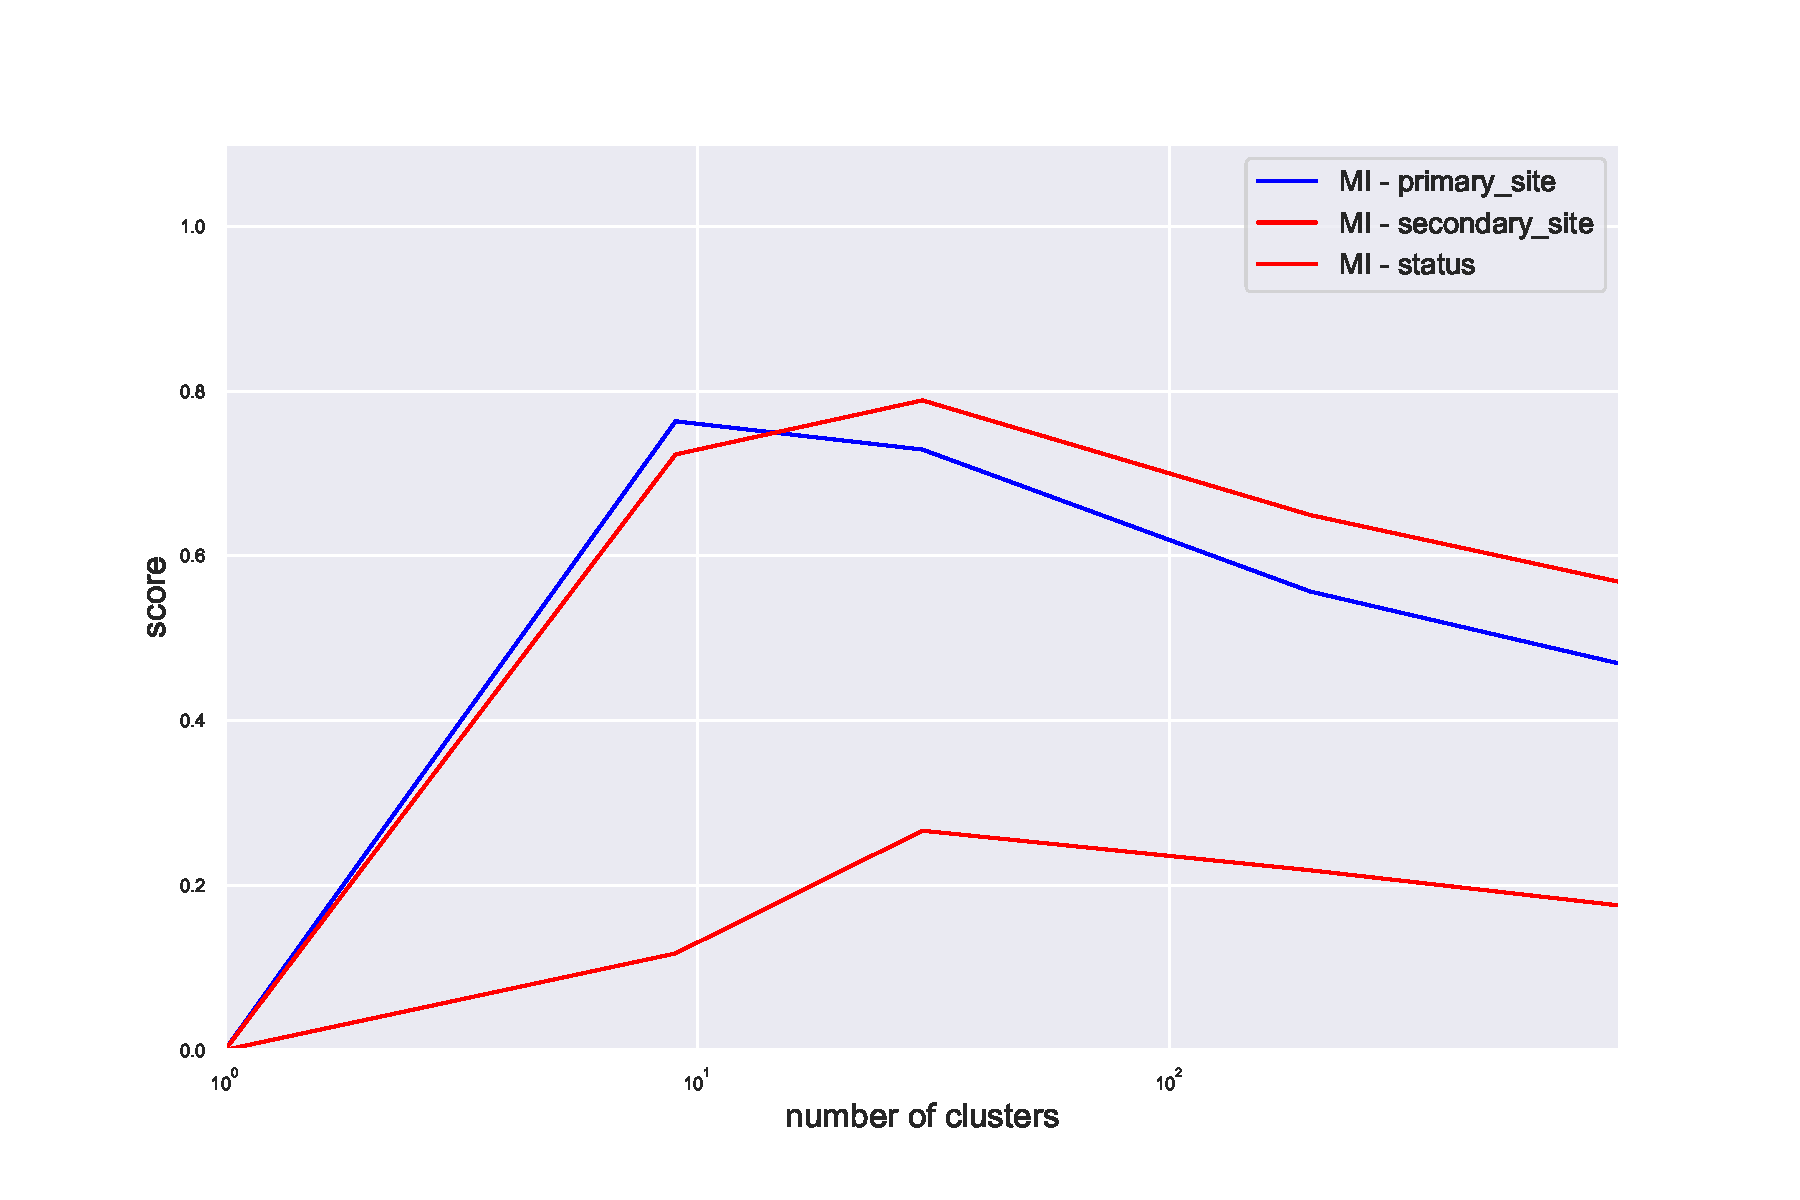
\includegraphics[width=0.8\linewidth]{pictures/topic/merged/metric_scores.pdf}
    \caption{V-measure score for run with merged healthy and diseased samples. Primary site (brain, blood, pancreas\ldots) labels are compared with secondary labels (healthy brain, brain cancer, healthy blood, blood cancer, healthy pancreas, pancreas cancer\ldots). The health status label (healthy / diseased) is plotted.}
    \label{fig:topic/merged/metric_scores}
\end{figure}
To conclude the score analysis a mixed score is considered (the homogeneity of primary site is considered with the completeness of secondary label) so that the score increase if going deeper in the hierarchy the separation of a homogeneous cluster brings to separation of the refined labels. In figure~\ref{fig:topic/merged/metric_scores_all} this score is compared with the one obtained with LDA, hierarchical clustering and the null model. What happened here is that hierarchical Stochastic Block Model performs the best, LDA approach is good, hierarchical clustering have a quite bad score and all are better than shuffling null model.
\begin{figure}[htb!]
    \centering
    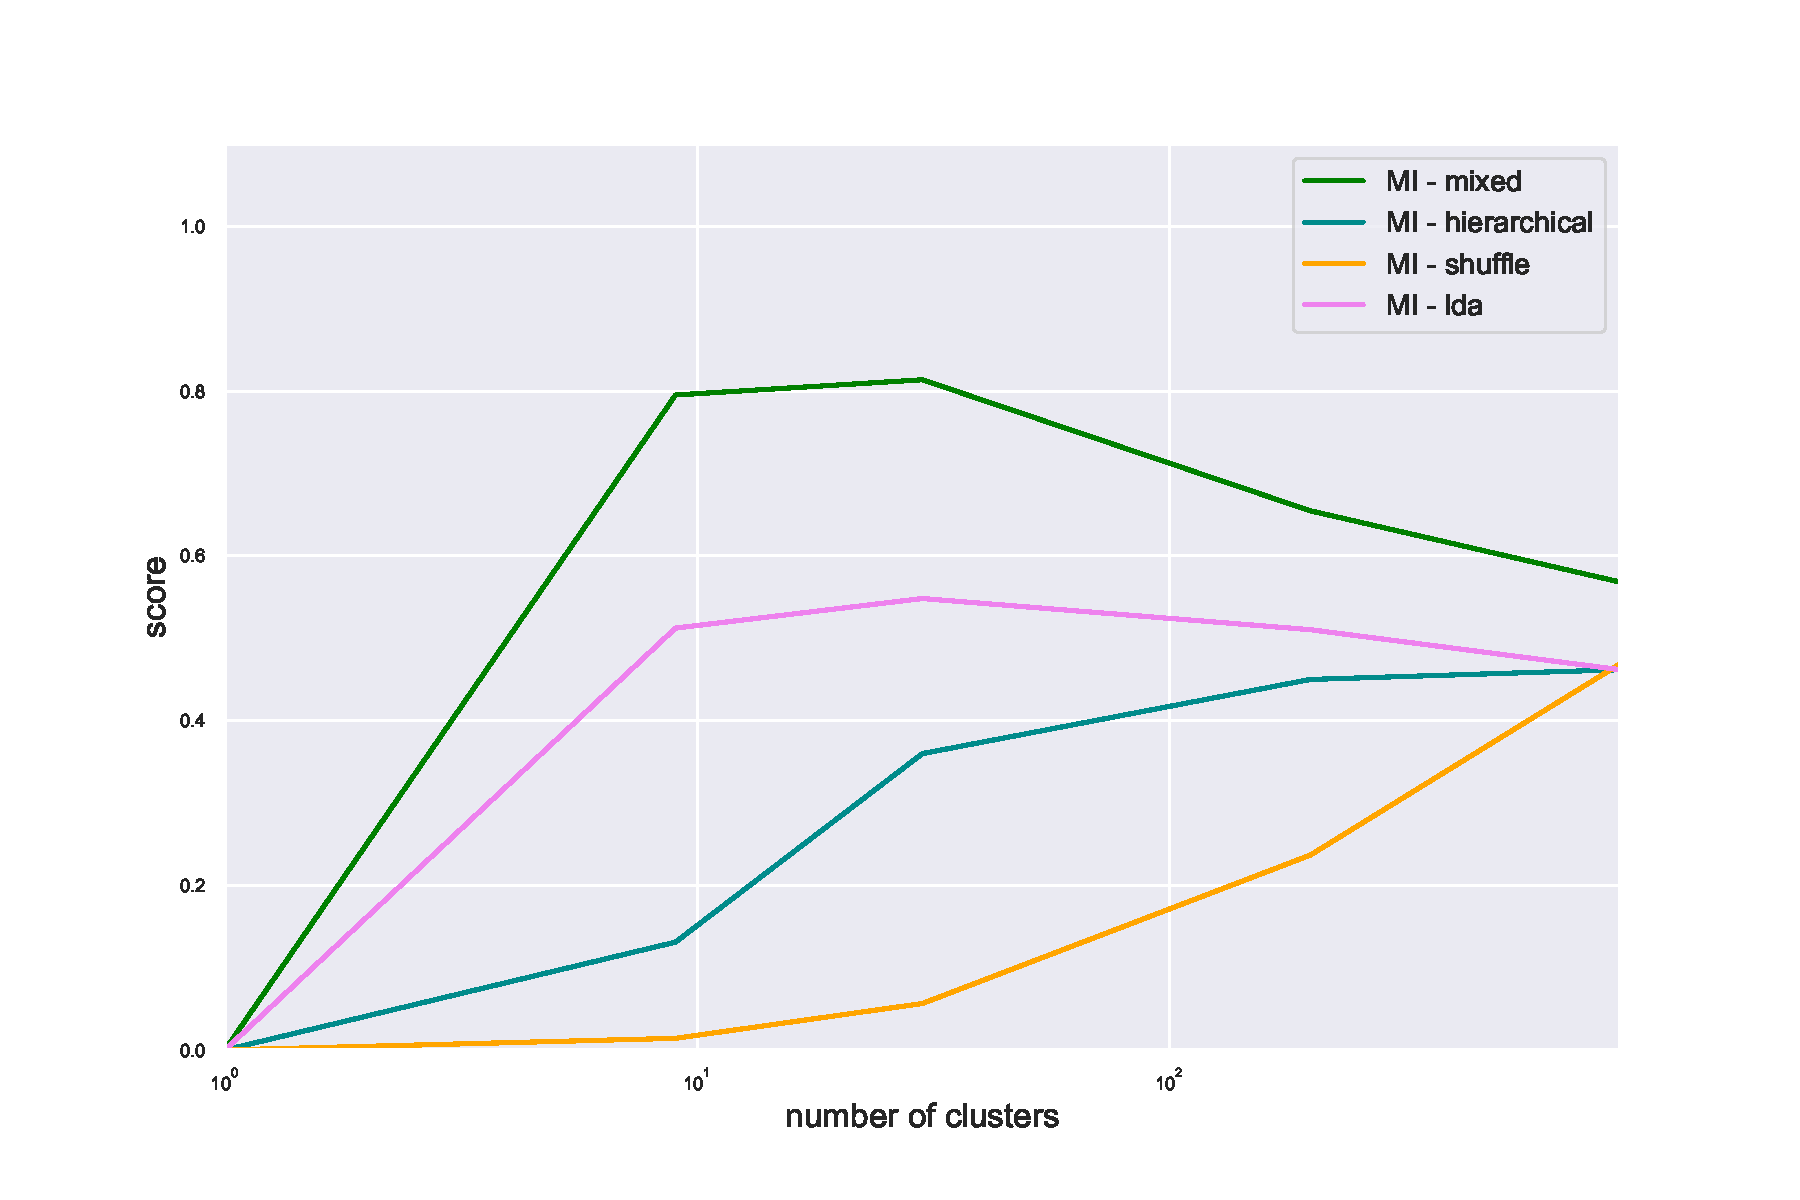
\includegraphics[width=0.8\linewidth]{pictures/topic/merged/metric_scores_all.pdf}
    \caption{V-measure score for run with merged healthy and diseased samples. LDA, hierarchical clustering and null model for comparison.}
    \label{fig:topic/merged/metric_scores_all}
\end{figure}

\FloatBarrier
\paragraph{Gene sets} analysis is then performed. Considering the P-value of the term which P-value was the lowest, one P-value for each topic at the level of the hierarchy where the V-measure was maximized, it is possible to realize the $-Log_{10}(\mathrm{P-value})$ histogram. The tests are quite interesting, in fact there is an enrichment with a P-value lower than $0.05$ in most cases so it is possible to assert that topics carry some interesting information more than expected by picking genes at random.
\begin{figure}[htb!]
    \centering
    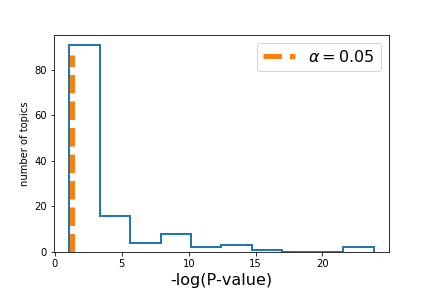
\includegraphics[width=0.5\linewidth]{pictures/topic/merged/pvaluescrosstopic.png}
    \caption{$-Log_{10}(\mathrm{P-value})$ of the term with the lowest P-value in each topic. In orange the standard $0.05$ threshold.}
    \label{fig:topic/merged/pvaluescrosstopic}
\end{figure}
In figure~\ref{fig:topic/merged/pvaluecategories} are shown the categories of the terms with lower P-values. This explains what aspect of the samples topic describes. The majority of terms found in topics comes from the GTEx annotation for tissue expression, many are from GO biological process, GO molecular function and some from Human phenotype ontology. 
\begin{figure}[htb!]
    \centering
    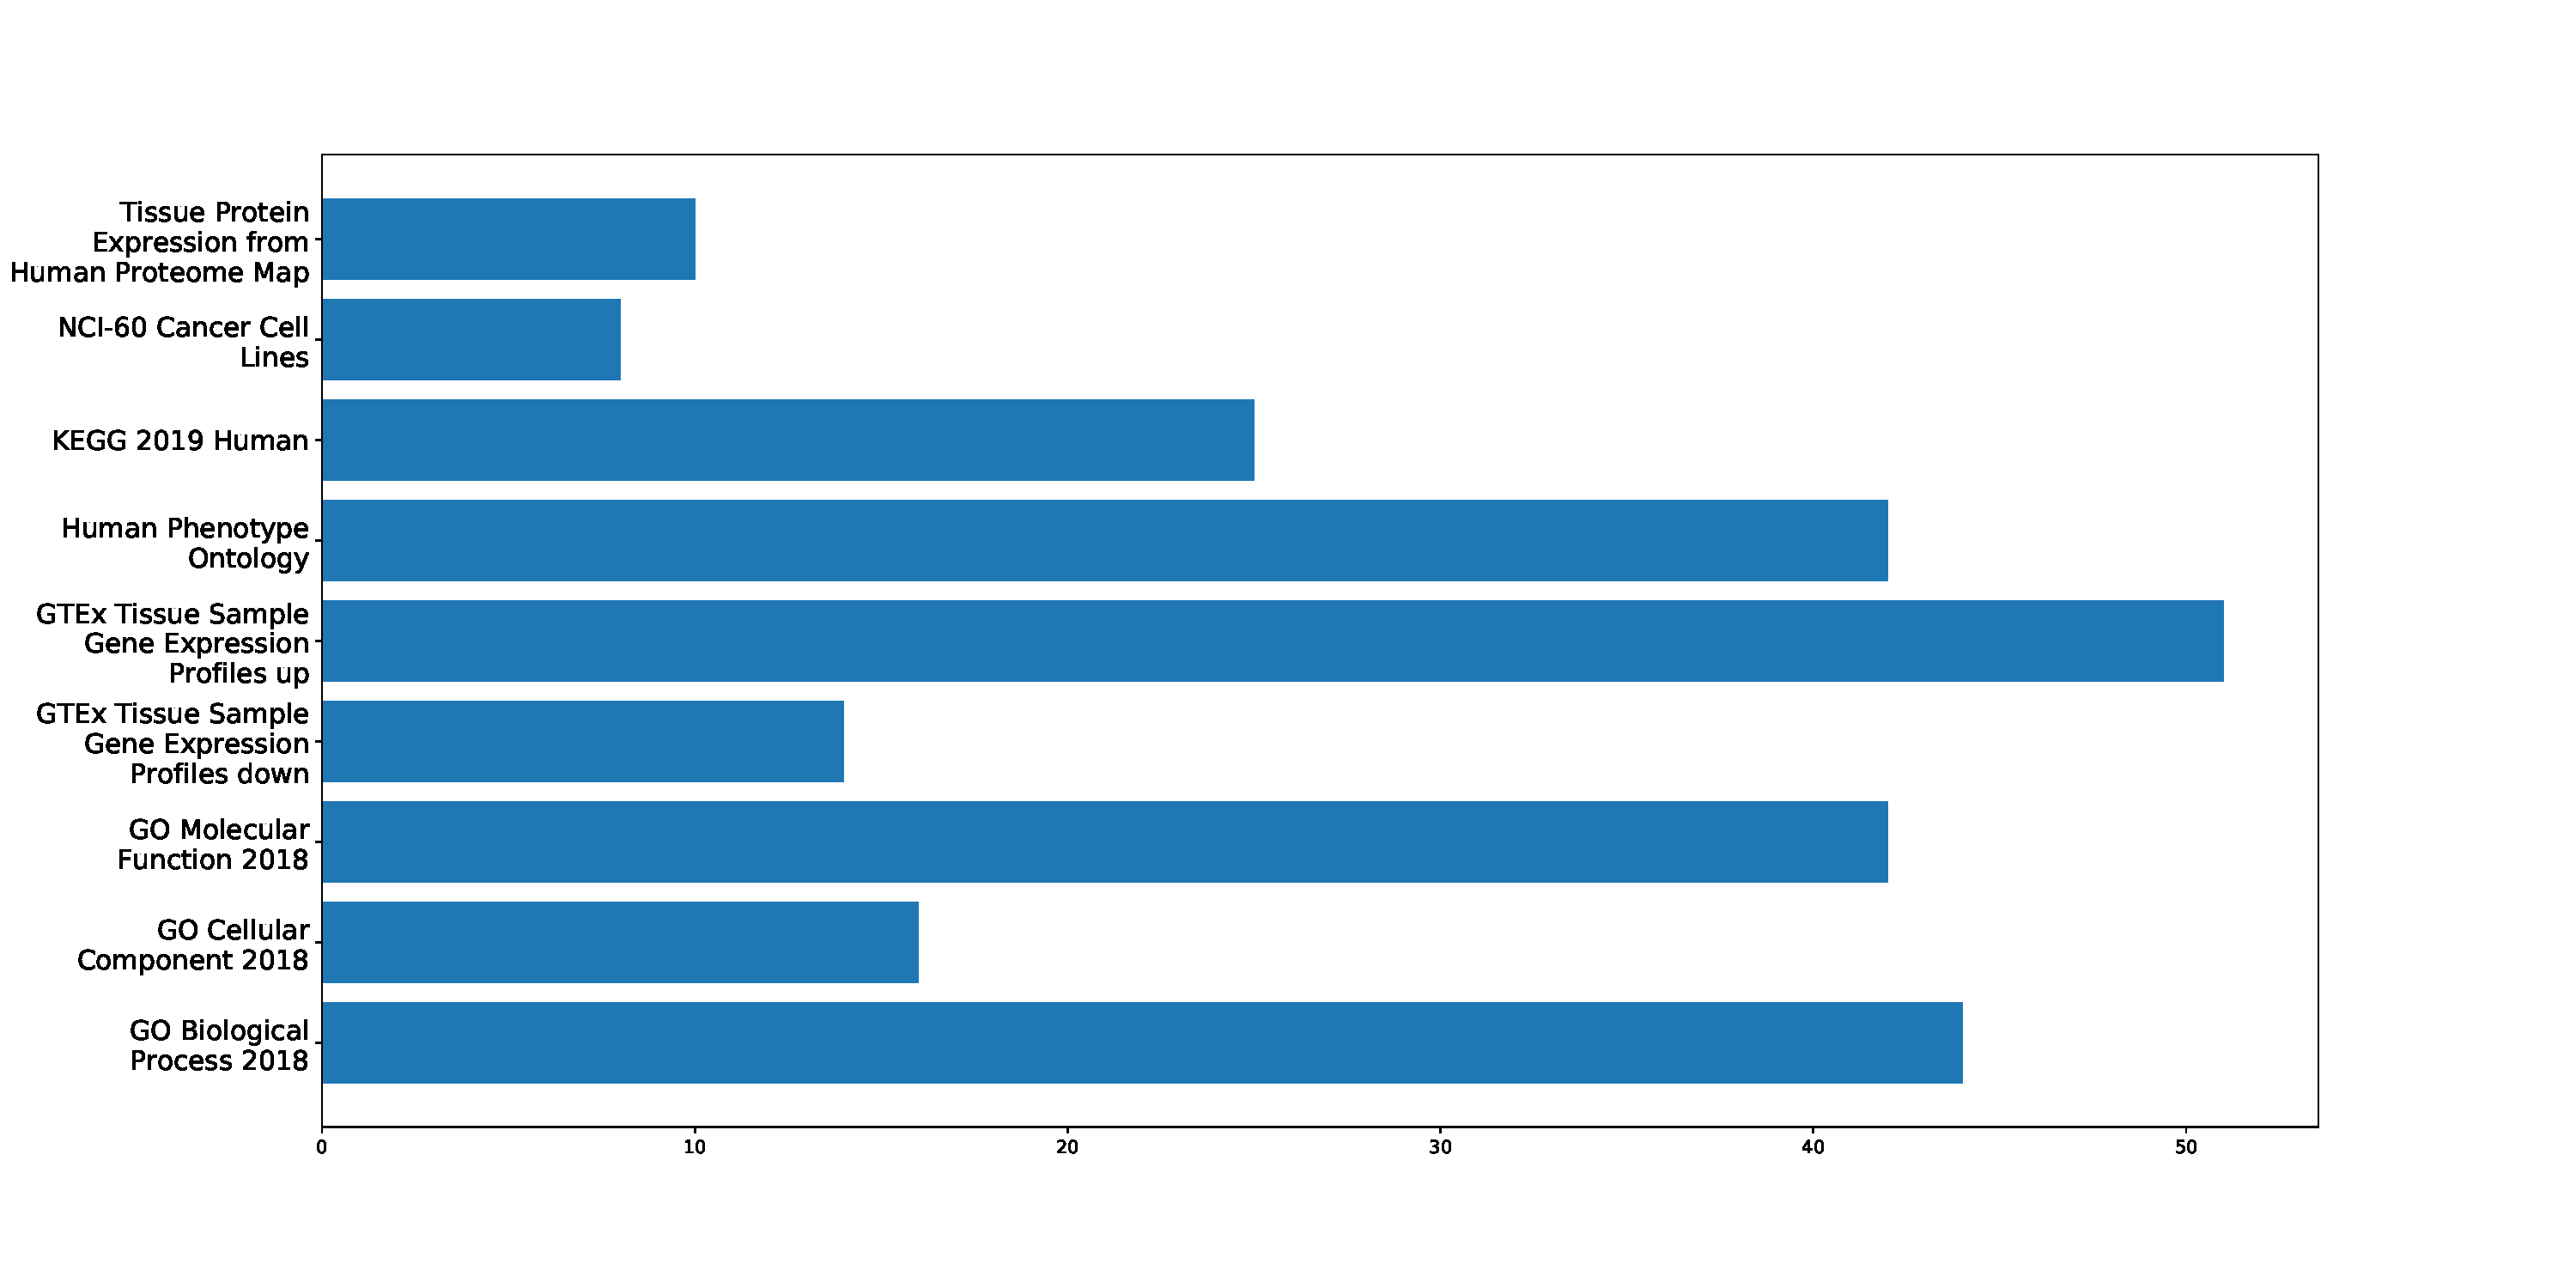
\includegraphics[width=0.8\linewidth]{pictures/topic/merged/pvaluecategories.pdf}
    \caption{Categories of the terms with lower P-values in each topic.}
    \label{fig:topic/merged/pvaluecategories}
\end{figure}

Going forward in the analysis it is possible to perform enrichment test with other tools such as DAVID~\cite{huang2008bioinformatics,huang2009systematic}. Results are similar to the ones retrieved before. Tissues related terms are found also using this tool and this confirms the absence of tool, sets, or categories related biases. In figures~\ref{fig:topic/merged/DAVID_lung},~\ref{fig:topic/merged/DAVID_brain} and ~\ref{fig:topic/merged/DAVID_stomach} the result from DAVID enrichment analysis. Finally, it is interesting to notice that topics are quite small (order $\simeq20$ genes), so there are no biases that can appear doing enrichment tests on big sets.
\begin{figure}[htb!]
    \centering
    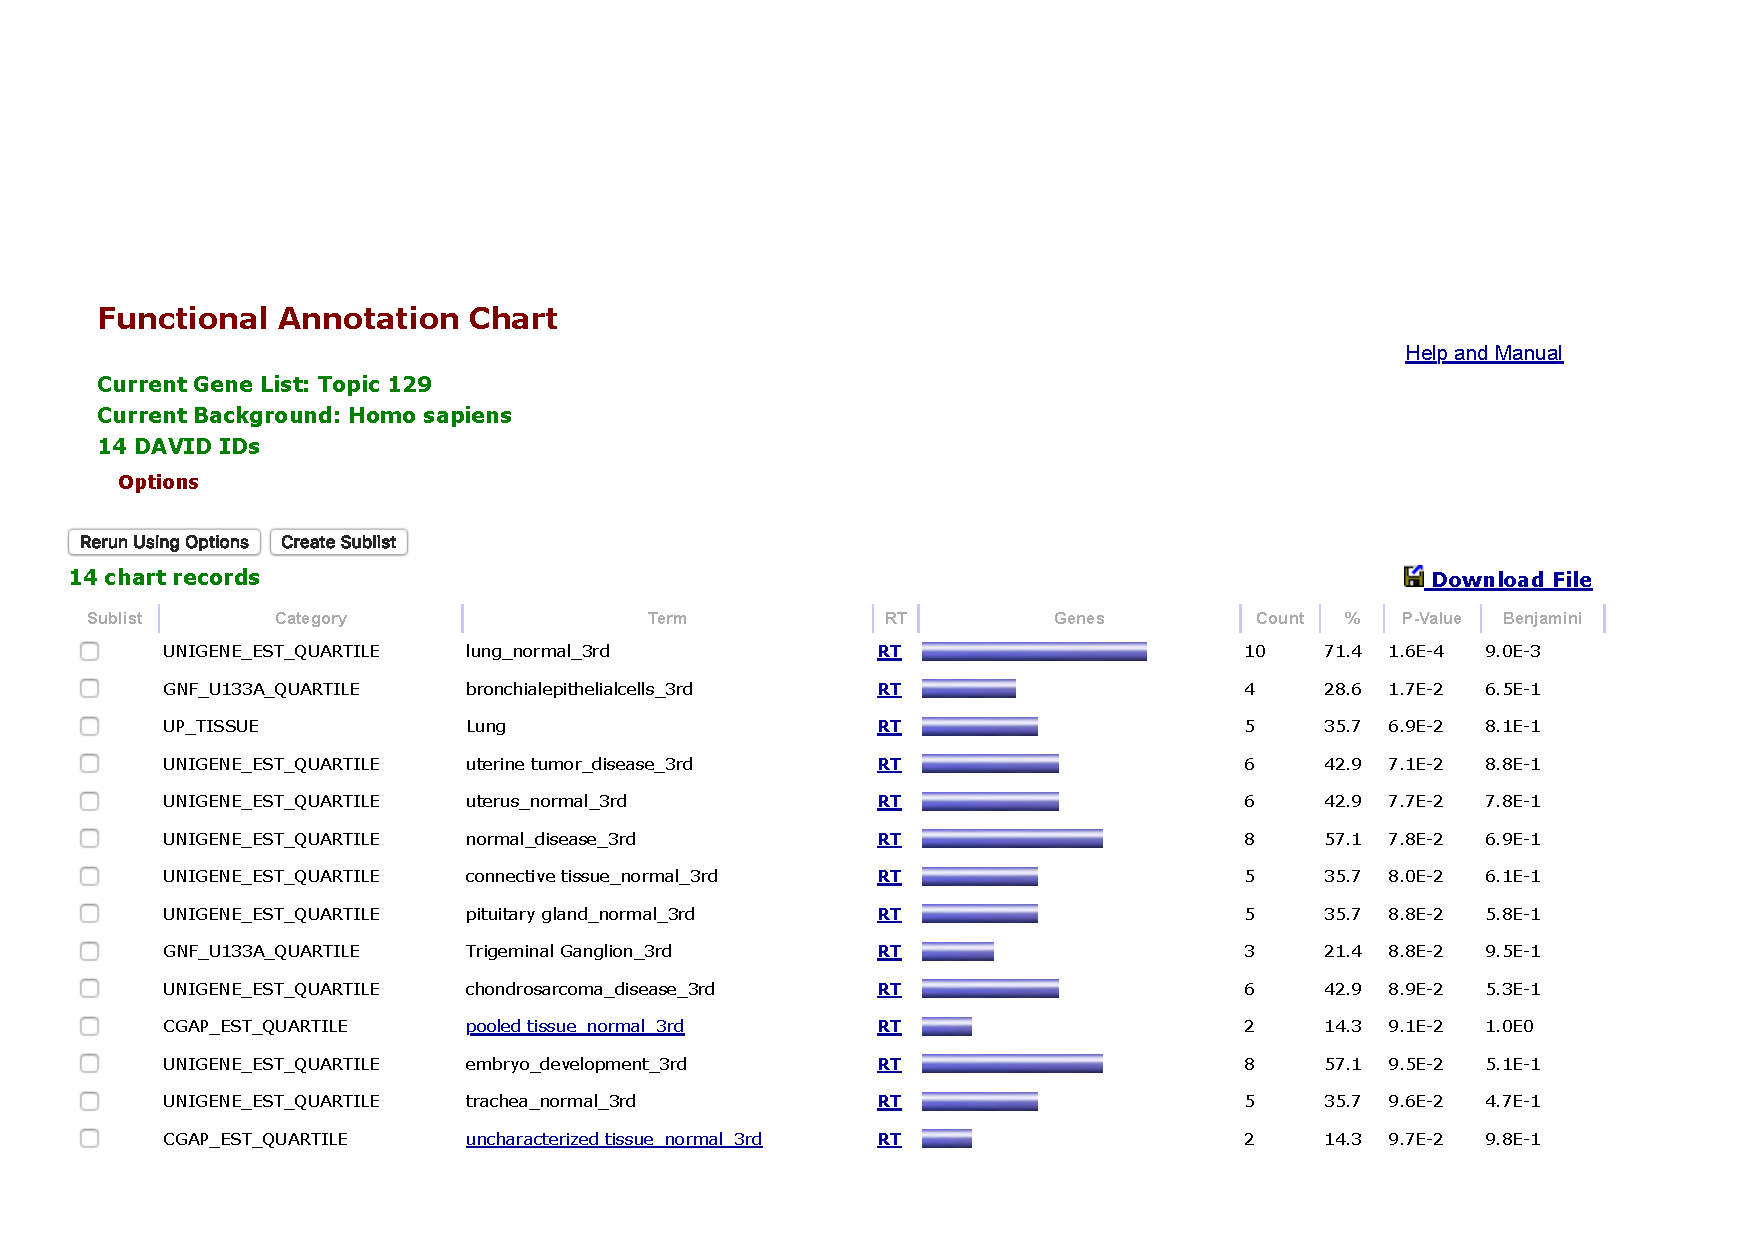
\includegraphics[width=0.6\linewidth]{pictures/topic/merged/DAVID_lung.pdf}
    \caption{Enrichment test on DAVID platform reveals lung related genes.}
    \label{fig:topic/merged/DAVID_lung}
\end{figure}
\begin{figure}[htb!]
    \centering
    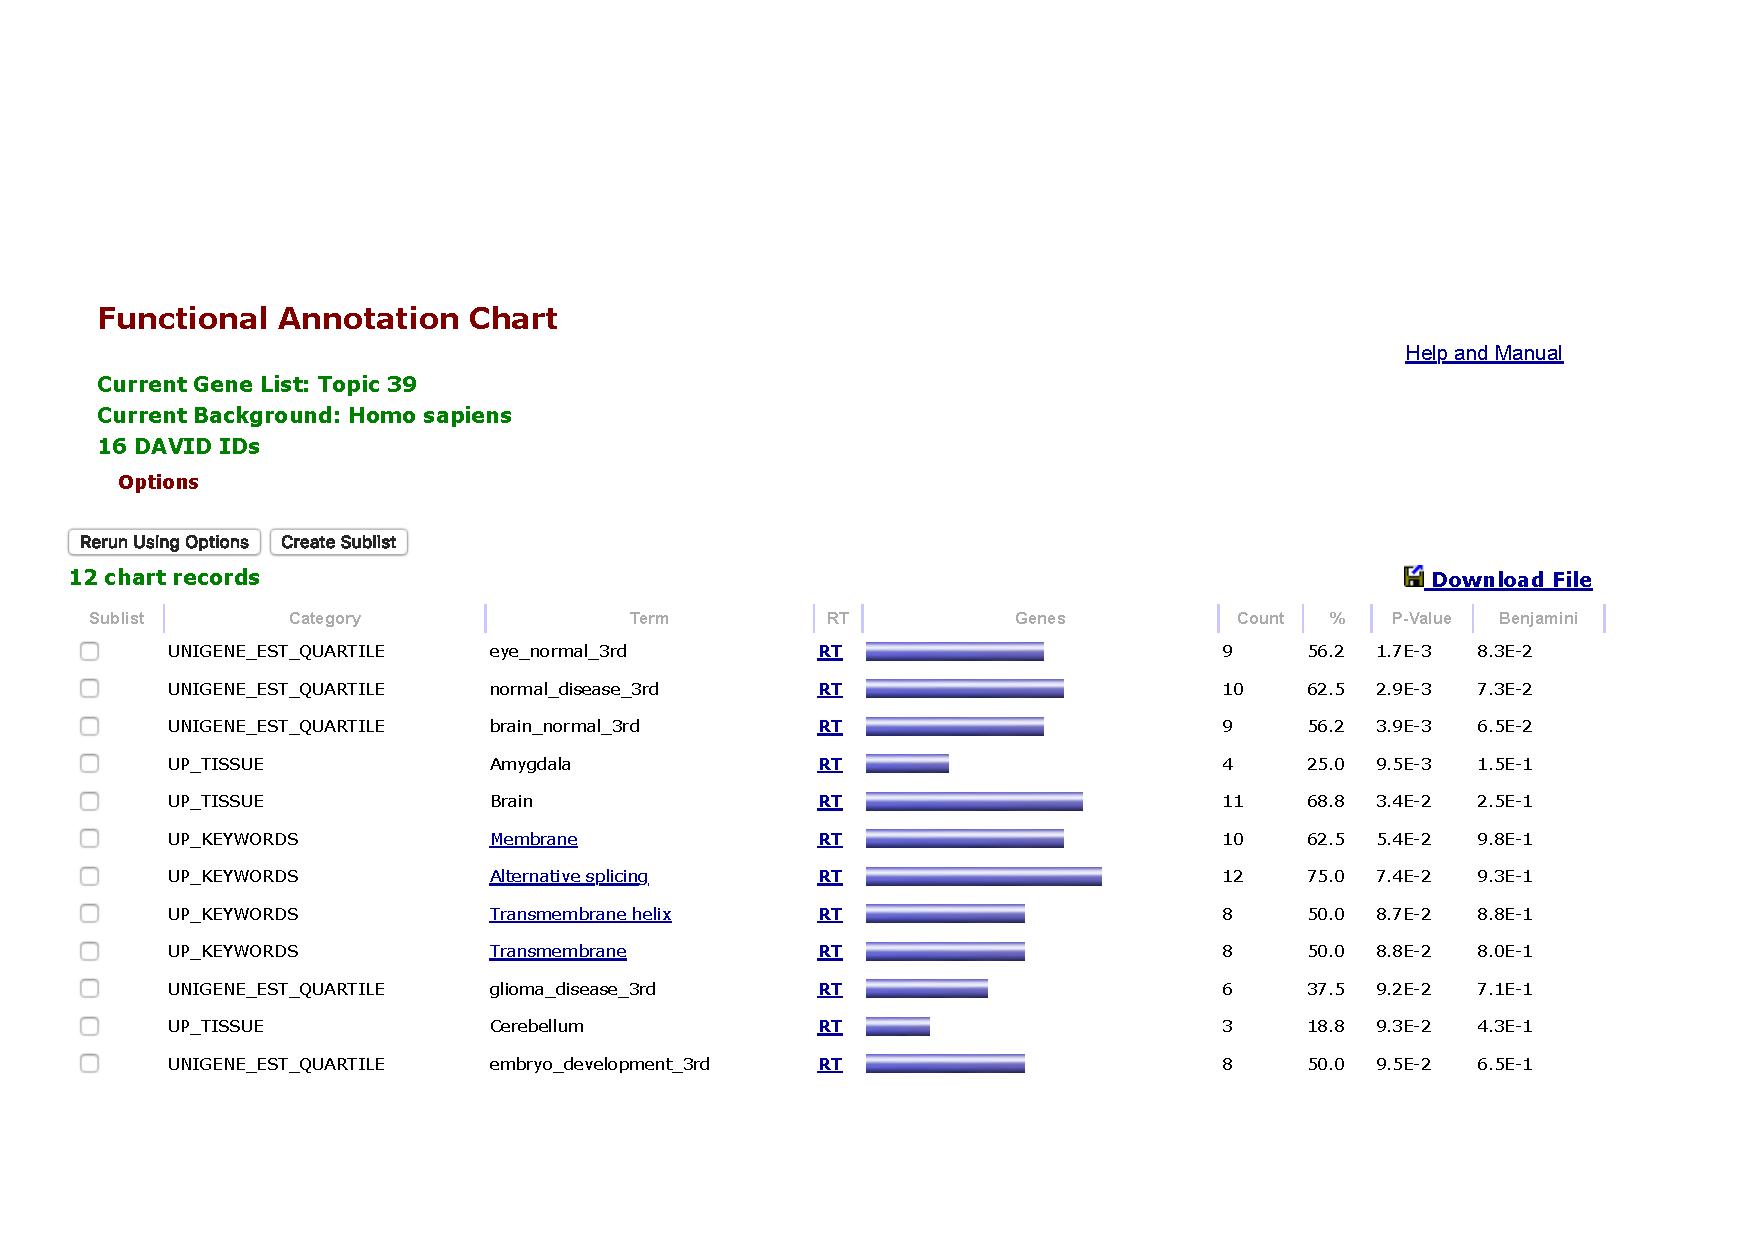
\includegraphics[width=0.6\linewidth]{pictures/topic/merged/DAVID_brain.pdf}
    \caption{Enrichment test on DAVID platform reveals brain related genes.}
    \label{fig:topic/merged/DAVID_brain}
\end{figure}
\begin{figure}[htb!]
    \centering
    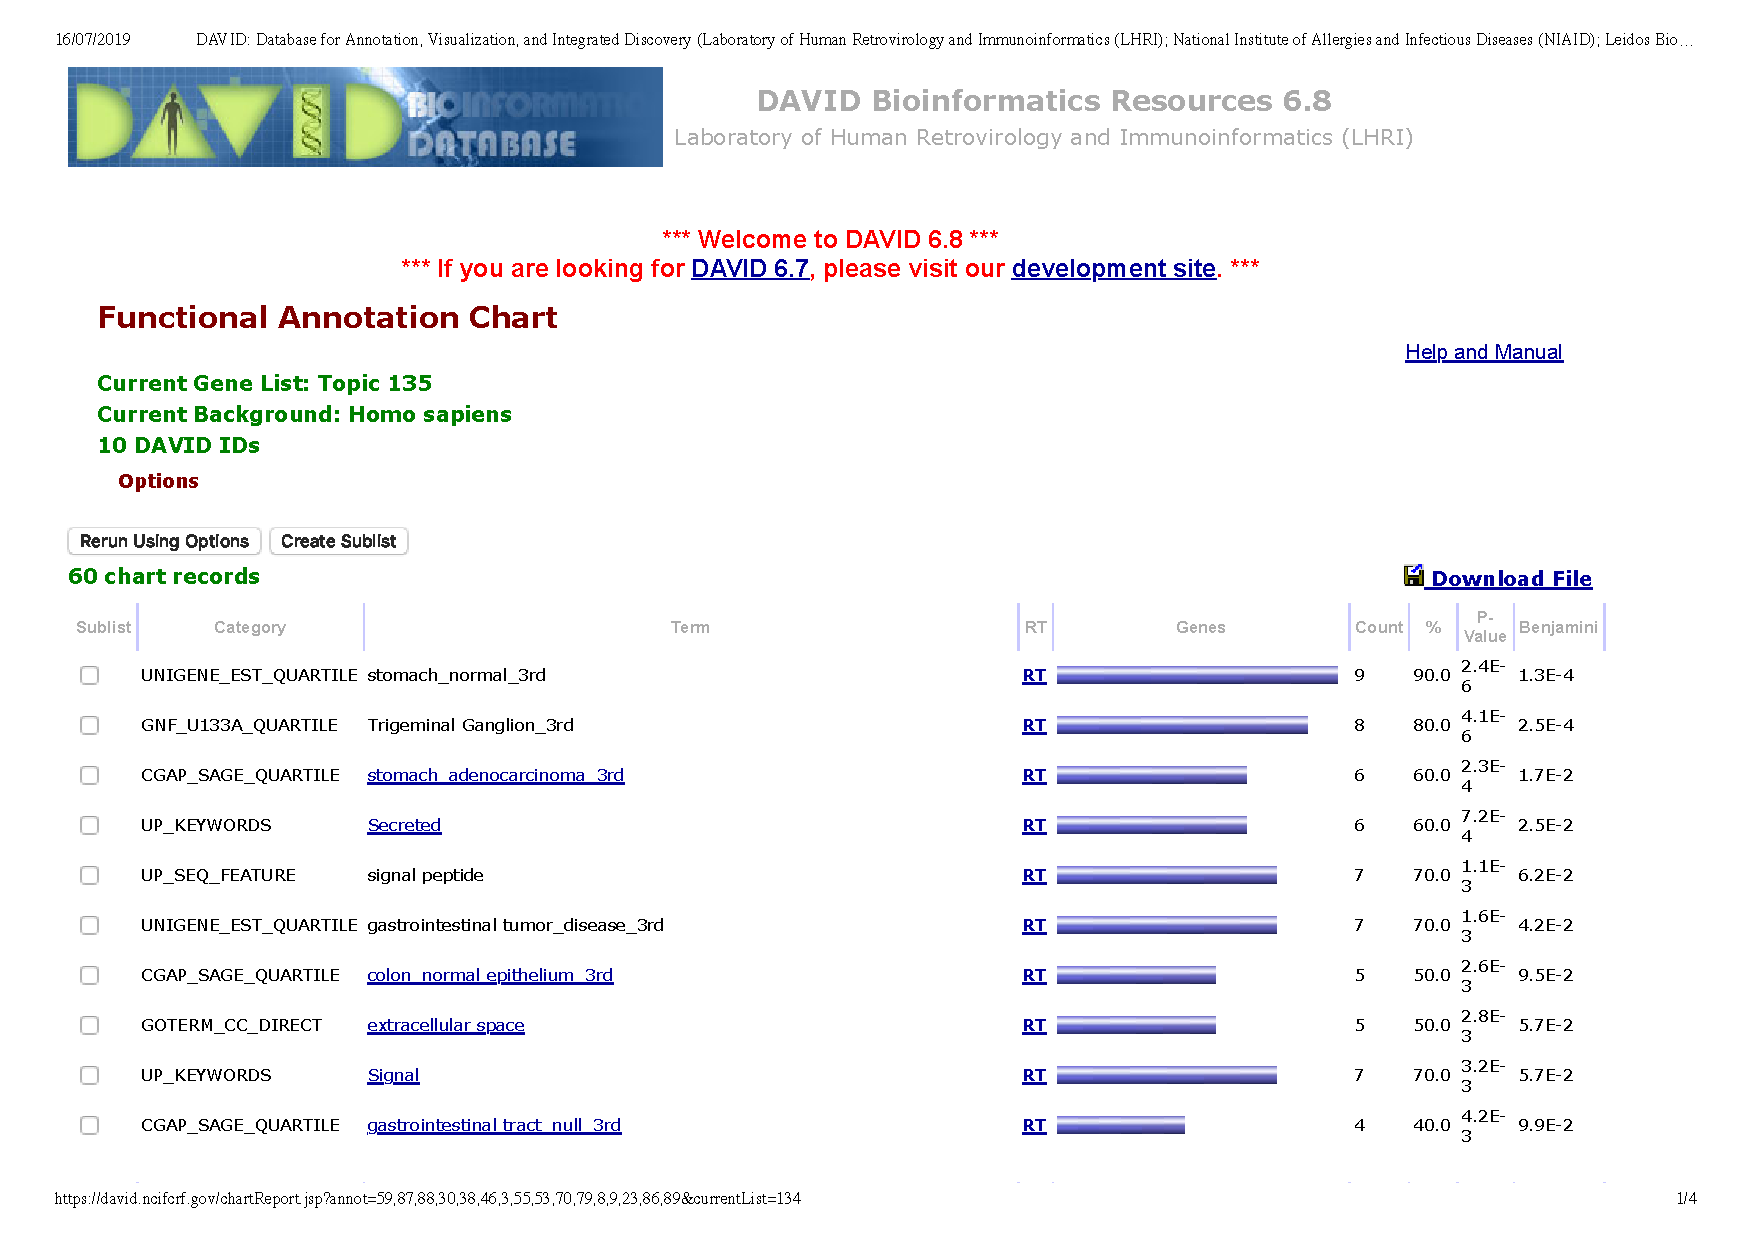
\includegraphics[width=0.6\linewidth]{pictures/topic/merged/DAVID_stomach.pdf}
    \caption{Enrichment test on DAVID platform reveals stomach related genes.}
    \label{fig:topic/merged/DAVID_stomach}
\end{figure}

\FloatBarrier
\paragraph{The link between topics and samples} has not been investigated so far. The probability distribution of each sample over topics $P(\text{topic}| \text{sample})$ can be estimated as \[P(\text{topic}| \text{sample})=\frac{\text{\# of edges on sample from topic}}{\text{\# of edges on sample}}\] after the model is run. Moreover, an average of all samples belonging to a topic can be estimated $P(\text{topic}| \text{tissue})=\frac{1}{\left|tissue\right|}\sum_{sample\in tissue}P(\text{topic}| \text{sample})$.

In figure~\ref{fig:topic/merged/lifeplot} it is plotted $P(\text{topic}| \text{tissue})$ for the first topics. What is clear is that in all samples there is a global trend that present no much differences between tissues, the topic expression differences between tissues are slightly appreciable at this point. This carries a profound and very informative message: under this new point of view in nature every tissue needs somehow the expression of all the genes (there is a global trend) and small differences between genes' expression are fine-tuned to obtain different tissues. In other words it is possible to describe human tissues assuming that all genes are important and that is the fine structure of their interactions which realizes the complexity observed. In the case of diseased samples this suggests that it should be possible to discover a cancer type not looking at a few marker genes but looking at the whole expression profile of all genes.
\begin{figure}[htb!]
	\centering
	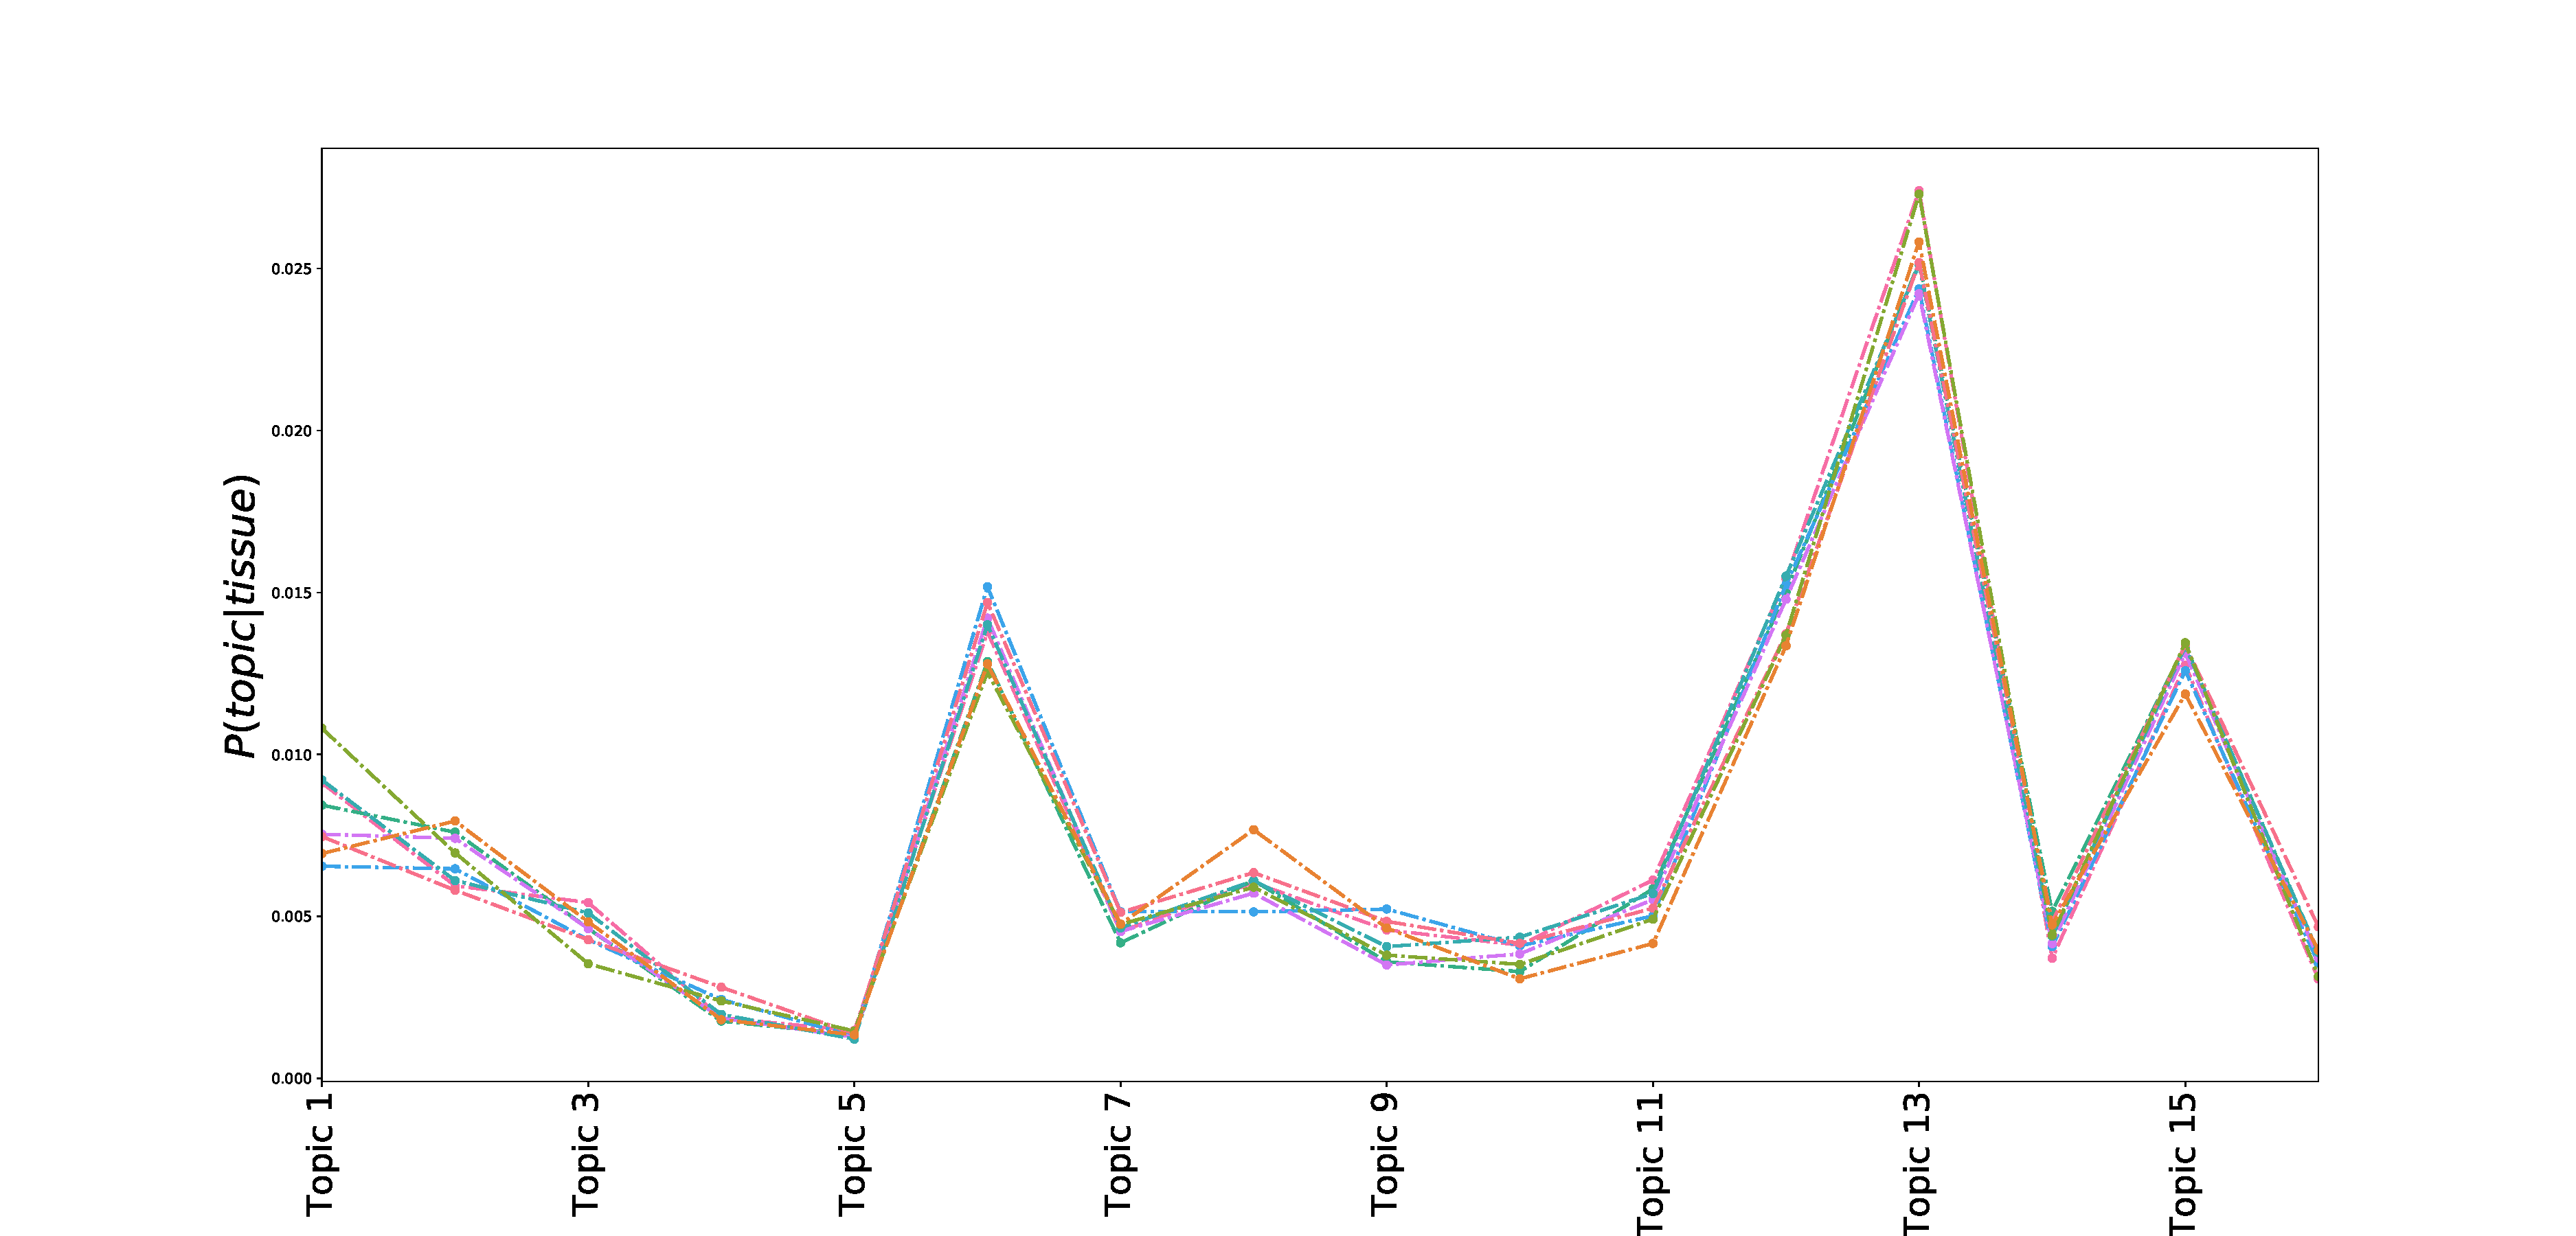
\includegraphics[width=0.9\linewidth]{pictures/topic/merged/lifeplot.pdf}
	\caption{$P(\text{topic} | \text{tissue})$ for some topic coloured by tissue. It is clear a global trend and in some topics there are little differences between tissues.}
	\label{fig:topic/merged/lifeplot}
\end{figure}

In order to better understand these differences between topic expression in different tissues some kind of normalization inside each topic is needed. Here it was chosen to study inside each topic which tissues are most differently expressed than average. To do so from each $P(\text{topic}| \text{tissue})$was subtracted the average topic expression $\text{mean}_{\text{tissue}}(\text{topic})=\avg{P(\text{topic}| \text{tissue})}_{tissue}$ and the result was divided by the standard deviation $\sigma_{\text{tissue}}(\text{topic})$. In figure~\ref{fig:topic/merged/lifeplot_normalised_level3_hd} some most characteristic topics are reported. This analysis reveals that tissue have a different behaviour than average in different topics, different tissues are distant from the average in different topics. This 
analysis is useful to determine what is the role of each topic, moreover if a topic reveals cancer the difference between the healthy tissue and its diseased counterpart emerges as shown in the figure.
\begin{figure}[htb!]
	\centering
	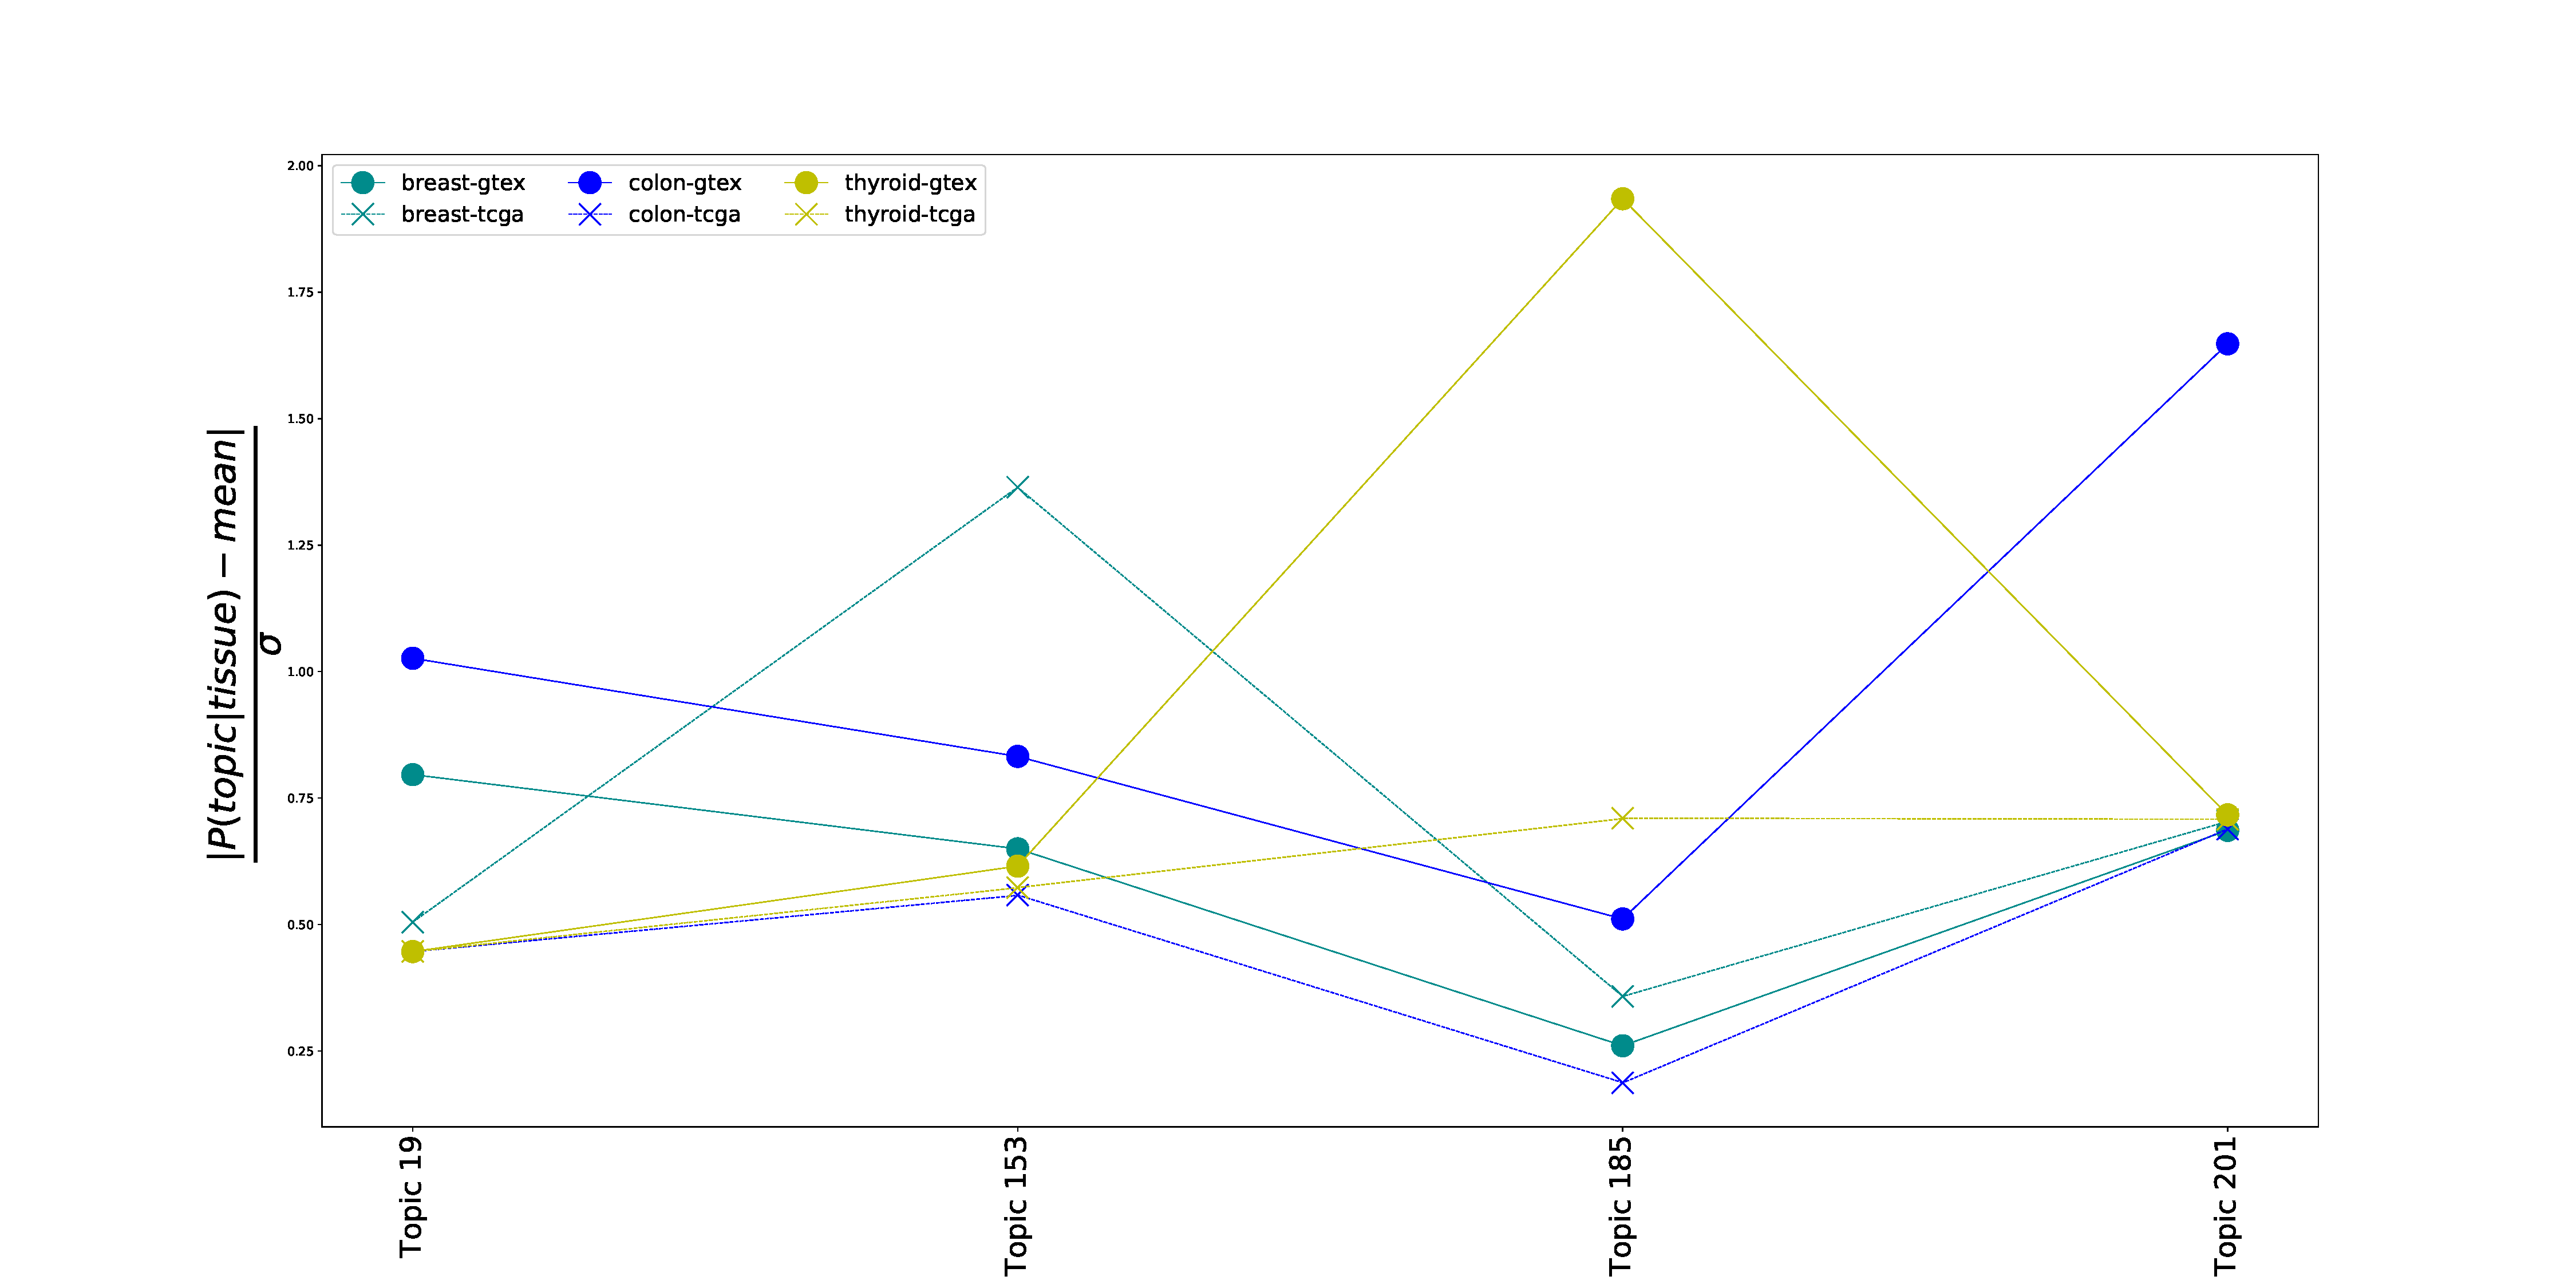
\includegraphics[width=0.85\linewidth]{pictures/topic/merged/lifeplot_normalised_level3_hd.pdf}
	\caption{$\frac{\left|P(topic | tissue) - \avg{P(\text{topic}| \text{tissue})}_{tissue}\right|}{\sigma_{\text{tissue}}(\text{topic})}$ or the distance of each tissue from the average tissue expression in each topic. Some low occurrence topics are reported.}
	\label{fig:topic/merged/lifeplot_normalised_level3_hd}
\end{figure}

The study of the relation between topics and samples conclude the topic modelling analysis. In the next section all results achieved will be summarized.